\documentclass[11pt,a4paper]{article}
\usepackage[margin=1in]{geometry}
\usepackage[T1]{fontenc}
\usepackage{lmodern}
\usepackage{microtype}
\usepackage{amsmath,amssymb,mathtools,bm}
\usepackage{booktabs,tabularx,array}
\usepackage{xcolor}
\usepackage{listings}
\usepackage{tikz}
\usetikzlibrary{arrows.meta,positioning,shapes.geometric,fit}
\usepackage[hidelinks]{hyperref}
\usepackage{enumitem}
\usepackage{caption}
\usepackage{float}
\setlist{nosep}
\definecolor{codebg}{RGB}{247,248,250}
\definecolor{codeblue}{RGB}{30,70,140}
\definecolor{codegreen}{RGB}{25,115,70}
\lstdefinestyle{python}{
  language=Python,
  basicstyle=\ttfamily\small,
  backgroundcolor=\color{codebg},
  keywordstyle=\color{codeblue}\bfseries,
  commentstyle=\color{codegreen},
  stringstyle=\color{red!65!black},
  numbers=left, numberstyle=\tiny\color{gray},
  breaklines=true, frame=single, rulecolor=\color{black!15},
  showstringspaces=false, columns=fullflexible
}
\title{Report 1: Foundations and Mathematical Principles of Grad-CAM}
\author{Technical Study Notes}
\date{\today}
\begin{document}
\maketitle
\tableofcontents
\newpage
\section{Introduction}
Gradient-weighted Class Activation Mapping (Grad-CAM) is a gradient-based technique for explaining the output of a differentiable neural network. It produces a coarse importance map at a selected internal layer. In this study, the target is an audio-enabled multimodal model whose audio tower processes a Mel-spectrogram and whose language-model head produces scores associated with Parkinson's disease (PD) and healthy control (HC).

The central question is: \emph{which positions in the selected audio representation provide positive evidence for the model's PD score relative to its HC score?} Grad-CAM answers this question with respect to a chosen scalar score and a chosen internal layer. It does not, by itself, establish that an acoustic feature is clinically causal.

\section{The model and the quantities being explained}
Let the input Mel-spectrogram be
\[
X\in\mathbb{R}^{M\times T_{\mathrm{in}}},
\]
where $M$ is the number of Mel-frequency bins and $T_{\mathrm{in}}$ is the number of spectrogram time frames. The audio tower transforms this input into hidden representations. At a selected layer, write the activation tensor as
\[
A\in\mathbb{R}^{B\times T\times D},
\]
where $B$ is batch size, $T$ is the number of audio-token positions, and $D$ is the hidden dimension. For one example, $A_{1,t,k}$ denotes feature channel $k$ at token position $t$.

The final language-model output is commonly represented by logits:
\[
Z\in\mathbb{R}^{B\times L\times V},
\]
where $L$ is the output sequence length and $V$ is vocabulary size. A logit is an unnormalized score for a vocabulary token at a particular sequence position.

\section{Choosing a scalar target score}
A gradient-based explanation needs a scalar objective. In the implementation, the selected objective is the difference between the PD and HC logits at the final sequence position:
\[
s=z_{\mathrm{PD}}-z_{\mathrm{HC}}.
\]
For a batch of one, this is implemented as
\[
s=Z[0,-1,\texttt{pd\_ids[0]}]
 -Z[0,-1,\texttt{hc\_ids[0]}].
\]
If $s>0$, the selected PD token has a larger logit than the selected HC token. If $s<0$, the selected HC token has the larger logit. This is a contrastive target: it asks what supports PD relative to HC, rather than what supports PD in isolation.

\subsection{Important tokenization qualification}
The code selects one vocabulary ID for each class. If a class label is split into multiple tokens, this expression does not automatically represent the probability of the complete label string. The prompt and tokenization must be checked. Also, the final-position logits predict the next token, so the prompt must be structured such that this next-token prediction is the intended classification decision.

\section{Gradients as local sensitivity}
The gradient of the score with respect to the activation tensor is
\[
G_{t,k}=\frac{\partial s}{\partial A_{t,k}}.
\]
It measures the local sensitivity of the selected score to a small change in one activation coordinate, holding the other coordinates fixed to first order. A positive value means that a small increase in that activation would locally increase $s$; a negative value means it would locally decrease $s$. A value near zero indicates low local sensitivity.

A first-order approximation makes this interpretation explicit:
\[
s(A+\Delta A)\approx s(A)+
\sum_{t=1}^{T}\sum_{k=1}^{D}
\frac{\partial s}{\partial A_{t,k}}\Delta A_{t,k}.
\]
This is a local differential statement, not proof of causation or a guarantee about large changes.

\section{Grad-CAM channel weights}
Grad-CAM aggregates gradients over spatial positions in image applications. In this audio-token setting, the corresponding position dimension is the token/time dimension. For each feature channel $k$, define
\[
\alpha_k=\frac{1}{T}\sum_{t=1}^{T}
\frac{\partial s}{\partial A_{t,k}}.
\]
The coefficient $\alpha_k$ is the average sensitivity of the score to channel $k$ across all token positions. It is a channel-level weight shared across positions.

For a batch of one, $G$ has shape $(1,T,D)$. Averaging over dimension $1$ with \texttt{keepdim=True} produces shape $(1,1,D)$, which can broadcast against the activation tensor $(1,T,D)$.

\section{The Grad-CAM map}
The pre-activation map at token position $t$ is
\[
C_t=\sum_{k=1}^{D}\alpha_k A_{t,k}.
\]
The conventional positive Grad-CAM map applies the rectified linear unit:
\[
L_t^{\mathrm{GradCAM}}=
\operatorname{ReLU}(C_t)=\max(0,C_t).
\]
The ReLU retains positive contributions to the selected target score under this Grad-CAM construction and suppresses negative values. Therefore, the resulting map is not a complete signed account of both positive and negative evidence. A separate signed or negative-evidence visualization would be needed to inspect those effects.

\section{Why both activations and gradients are needed}
Activations describe what representation is present at a position. Gradients describe how sensitive the target score is to that representation. Grad-CAM combines the two:
\[
L_t^{\mathrm{GradCAM}}=
\operatorname{ReLU}\left(
\sum_k
\underbrace{\left(\frac{1}{T}\sum_{u=1}^{T}
\frac{\partial s}{\partial A_{u,k}}\right)}_{\text{channel importance}}
\underbrace{A_{t,k}}_{\text{local activation}}
\right).
\]
Using activations alone would not indicate their relationship to the selected score. Using gradients alone would not incorporate the magnitude of the features present at each position.

\section{Forward hooks and gradient retention}
A PyTorch forward hook is a callback executed when a particular module completes its forward computation. It receives the module, its input, and its output. In the implementation, the hook extracts the hidden-state tensor and stores it.

\begin{lstlisting}[style=python]
def forward_hook(module, inp, output):
    activation = output[0] if isinstance(output, tuple) else output
    activations.append(activation)
    activation.retain_grad()
\end{lstlisting}

The hook captures the activation during the forward pass; it does not calculate the gradient. The call \texttt{retain\_grad()} asks PyTorch to retain the gradient on this non-leaf tensor after backpropagation. PyTorch normally populates the \texttt{.grad} attribute automatically for leaf tensors, but not for most intermediate tensors.

After the scalar score has been computed, calling \texttt{score.backward()} propagates derivatives through the computation graph. The retained gradient can then be read from \texttt{activation.grad}. Retention does not create a gradient if the activation is disconnected from the score, or if gradient tracking is disabled.

\section{Conceptual execution order}
\begin{figure}[H]
\centering
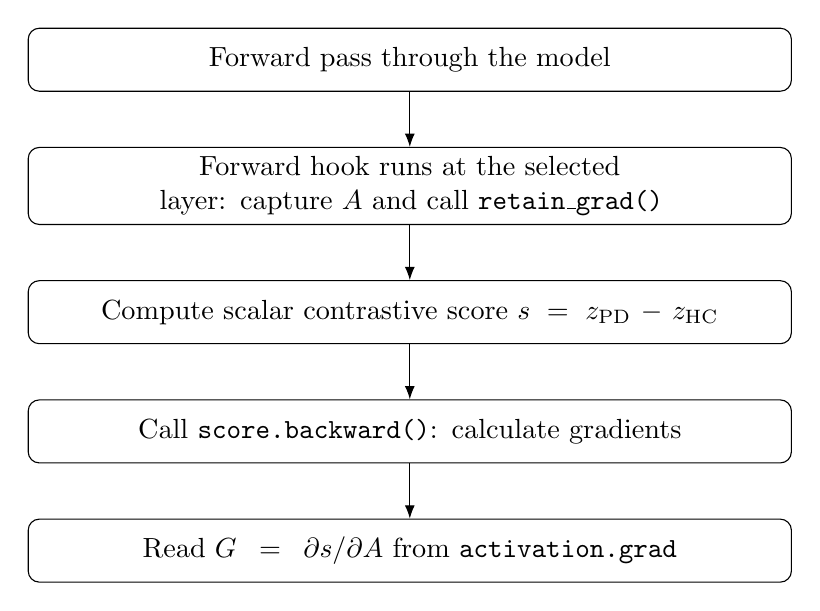
\begin{tikzpicture}[node distance=7mm, every node/.style={draw,rounded corners,align=center,
text width=0.78\linewidth,minimum height=8mm}, >=Latex]
\node (f) {Forward pass through the model};
\node (h) [below=of f] {Forward hook runs at the selected layer: capture $A$ and call \texttt{retain\_grad()}};
\node (s) [below=of h] {Compute scalar contrastive score $s=z_{\mathrm{PD}}-z_{\mathrm{HC}}$};
\node (b) [below=of s] {Call \texttt{score.backward()}: calculate gradients};
\node (g) [below=of b] {Read $G=\partial s/\partial A$ from \texttt{activation.grad}};
\draw[->] (f)--(h); \draw[->] (h)--(s); \draw[->] (s)--(b); \draw[->] (b)--(g);
\end{tikzpicture}
\caption{The hook captures the activation during the forward pass; backpropagation computes its gradient later.}
\end{figure}

\section{Selecting the target layer}
The expression
\begin{lstlisting}[style=python]
target_layer = model.model.audio_tower.layers[-1]
\end{lstlisting}
selects the last module in the audio tower's \texttt{layers} sequence. Python index \texttt{-1} means the final element. It does not mean the first output or first activation. The later expression \texttt{output[0]} is a separate operation: if the module returns a tuple, it selects the tuple's first element. The code assumes that this first element is the hidden-state tensor of interest. This assumption should be verified by inspecting the module's output structure and tensor shape.

\section{Assumptions and limitations}
\begin{enumerate}
\item The chosen layer must execute during the forward pass and its output must lie on a differentiable path to the score.
\item The tuple-handling rule assumes the first tuple element is the desired hidden state. Different architectures may return different structures.
\item The score explains a particular logit contrast at a particular sequence position, not every aspect of the model's decision.
\item Grad-CAM is layer-dependent and coarse. Its map should not be interpreted as a pixel- or frequency-exact attribution.
\item Positive Grad-CAM values indicate positive evidence under this construction, not clinical causality.
\end{enumerate}

\section{Summary}
Grad-CAM for the audio model consists of selecting an internal audio representation, capturing its activation, defining a scalar PD-versus-HC score, differentiating that score with respect to the activation, averaging gradients over audio-token positions, and combining the resulting channel weights with the activations. The forward hook captures and retains the activation; the later backward pass computes the gradient.

\end{document}
